\documentclass[11pt]{article}
\usepackage[margin=1in]{geometry}
\usepackage{setspace}
\usepackage{natbib}
\usepackage{hyperref}
\usepackage{graphicx}
\usepackage[switch]{lineno}
\hypersetup{colorlinks=true,linkcolor=blue,citecolor=blue,urlcolor=blue}
\setstretch{1.15}

\title{The BIEN Species App: A species-level interface for exploring occurrence, trait, and range evidence}
\author{
Brian J. Enquist$^{1}$ \\ 
Cory Merow$^{2}$
}
\date{\today}

\begin{document}
\maketitle
\noindent $^{1}$ Department of Ecology and Evolutionary Biology, University of Arizona, Tucson, AZ, USA \\
\noindent $^{2}$ Eversource Energy Center and Department of Ecology and Evolutionary Biology, University of Connecticut, Storrs, CT, USA

\linenumbers

\section*{Abstract}
Modern biodiversity studies rely on large shared databases, but researchers often jump from data download straight to modeling. The BIEN Species Shiny App adds an important middle step: a clear, visual check of what the data actually look like for a species. Users enter a scientific name and see linked views of occurrence points, trait records, and range layers from BIEN. The app helps answer practical questions quickly: Where are records concentrated? Which source types dominate? How do filter choices change results? Are range layers available when point coordinates are sparse? The design keeps key decisions visible, including native versus introduced filters, cultivated versus wild filters, and coordinate-quality filtering. It also shows when fallback query settings were needed to return records. By focusing on data source and uncertainty---not just record totals---the app supports better decisions before formal analyses. This article explains what the app does, how to use it, and how it can improve transparent reporting in BIEN-based ecological workflows.

\section*{Introduction}
Large biodiversity resources have changed ecology by making species records and traits much easier to access \citep{Enquist2026BIEN, Maitner2025BIEN}. But putting many sources into one system does not remove interpretation problems. Researchers still need to know whether records are clustered in a few places, whether observations are mainly museum specimens or casual sightings, whether introduced records matter for the question, and whether trait values are sparse or reported in mixed units. In practice, these checks are often done informally and are not reported in a consistent way.

The BIEN Species Shiny App addresses this gap with a lightweight interface for species-level data checking. It is not a replacement for modeling tools. Instead, it is an early decision step that helps users choose whether and how to continue to formal analysis. This fits a core recommendation in ecological methods: examine assumptions and data limits before fitting models \citep{Merow2013MaxEntGuide, Merow2014Maxlike, Merow2016ExpertMaps}.

The app is built in R using \texttt{shiny}, \texttt{leaflet}, \texttt{DT}, \texttt{dplyr}, \texttt{stringr}, and \texttt{sf} \citep{Chang2024Shiny, Cheng2024Leaflet, Xie2024DT, Wickham2023Dplyr, Wickham2023Stringr, Pebesma2018SF}. It queries BIEN and presents results in linked tabs so users can move smoothly between occurrence mapping, community-focused plot/survey mapping, observation-source tables, trait summaries/graphics, range context, and downloadable data/code outputs \citep{Maitner2025BIEN}. The aim is practical: make species-level data inspection fast, understandable, and repeatable, even for users who are not writing complex code.

\section*{What the app does}
\subsection*{Species-level occurrence exploration}
At its core, the app runs a BIEN occurrence query from a species name and shows results in an interactive map and searchable table. The map is designed for readability rather than maximum point count. If there are many records, users can balance the displayed subset by source type so one stream does not visually dominate the page. This is especially useful for common species, where a single source can otherwise give a misleading first impression.

The table gives the matching row-level details. Users can inspect source fields, coordinate columns, and taxonomy fields, then compare table content with the map. This linked view reduces a common mistake in exploratory work: making conclusions from the map alone.

\subsection*{Transparent filtering and fallback logic}
A key feature is that important biological filters are visible and easy to change. Users can control introduced versus native handling, cultivated versus wild inclusion, coordinate-quality filtering, and optional exclusion of field-observation/citizen-science streams. A conservative default profile (native-only, cultivated excluded, geovalid-only) is available for quick ecological screening.

The app also uses clear fallback query steps. If strict settings return no usable data, it relaxes filters in a defined order (for example, relaxing native-only or coordinate-quality constraints) and records which step produced results. Users can therefore see not just \emph{that} records appeared, but also under which settings.

\subsection*{Observation-source interpretation}
Raw source fields in large occurrence infrastructures are often difficult to interpret quickly. To support rapid triage, the app derives broad observation categories from BIEN provenance fields, including specimen/herbarium, plot/survey, iNaturalist-linked citizen science, HumanObservation field records, and GBIF/other aggregator classes. This does not replace formal Darwin Core harmonization \citep{Wieczorek2012DarwinCore}, but it provides immediate context about record streams likely to differ in sampling process and uncertainty profile.

The distinction between categories is intentionally conservative. For example, GBIF is treated as an aggregator category rather than automatically as citizen science, because aggregated datasets can include preserved specimens, inventories, and observations. Likewise, the HumanObservation category can include both crowd-sourced and expert field records, so exclusions should be interpreted carefully.

\subsection*{Community (plot/survey) view}
The Community tab focuses specifically on records categorized as plot/survey observations. It maps those records separately from the full occurrence view and reports concise summary statistics below the map (for example, number of plot/survey rows, mappable points, source and dataset breadth, and temporal span when available). This gives users a fast way to assess community-style evidence without manually filtering the larger occurrence table.

\subsection*{Trait and range evidence}
The app retrieves BIEN trait records and shows both raw rows and compact summaries by trait name and unit. Numeric values are plotted as histograms in a dedicated graphics tab, while non-numeric or mixed-format values remain in tables. This makes it easier to judge whether trait data are ready for quantitative analysis or better used as descriptive evidence.

For species with few usable coordinates but available BIEN range layers, users can load and map those layers on demand. This is intentional: range products can be useful context, but they are not direct substitutes for point records. Showing both in one interface helps users keep that distinction clear.

\begin{figure}[htbp]
\centering
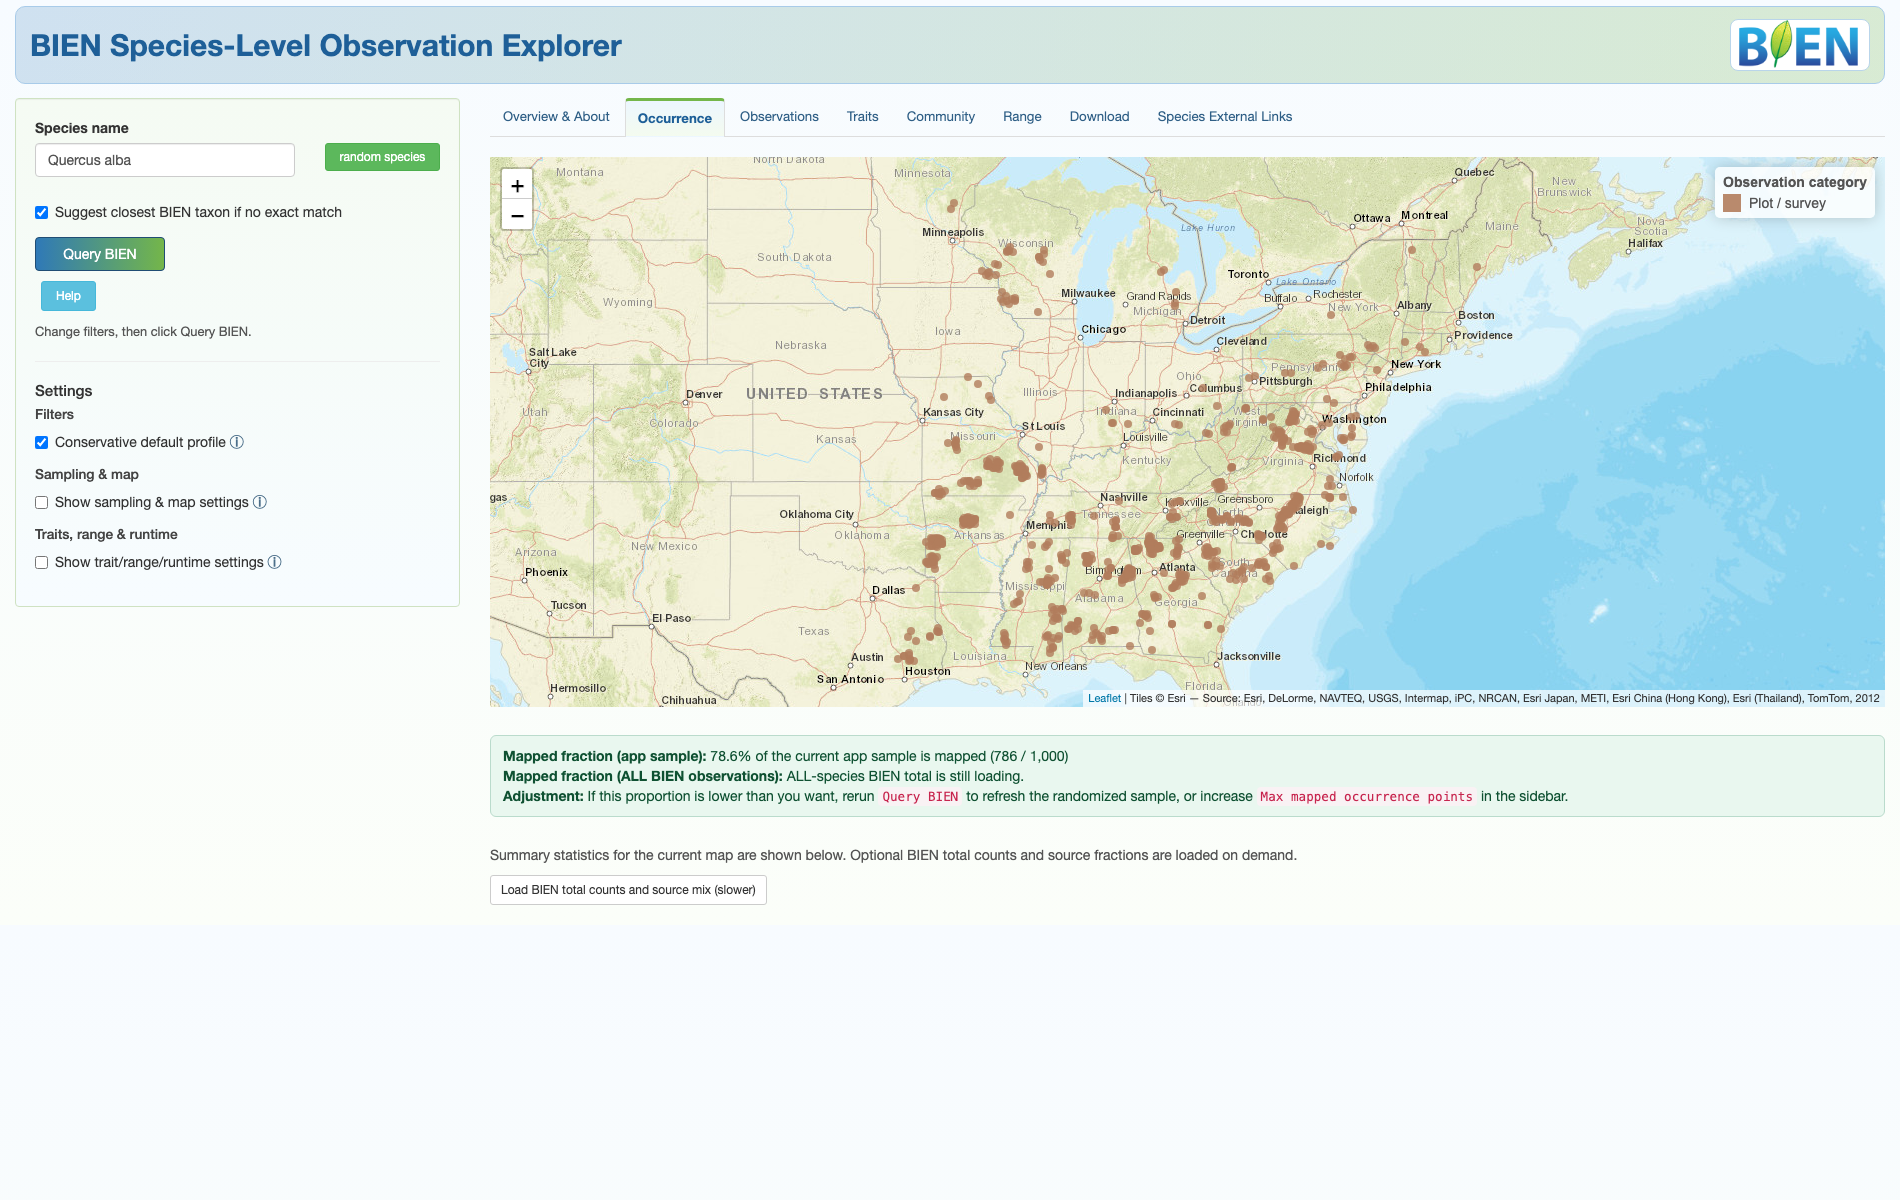
\includegraphics[width=\textwidth,height=0.78\textheight,keepaspectratio]{figures/fig_occurrence_map.png}
\caption{Occurrence Map view of the BIEN Species Shiny App for \textit{Pinus ponderosa} (locked screenshot species). The figure shows populated occurrence records, source-aware map rendering, and the filter panel used to control native status, cultivated status, and coordinate-quality settings.}
\label{fig:occurrence_map}
\end{figure}

\begin{figure}[htbp]
\centering
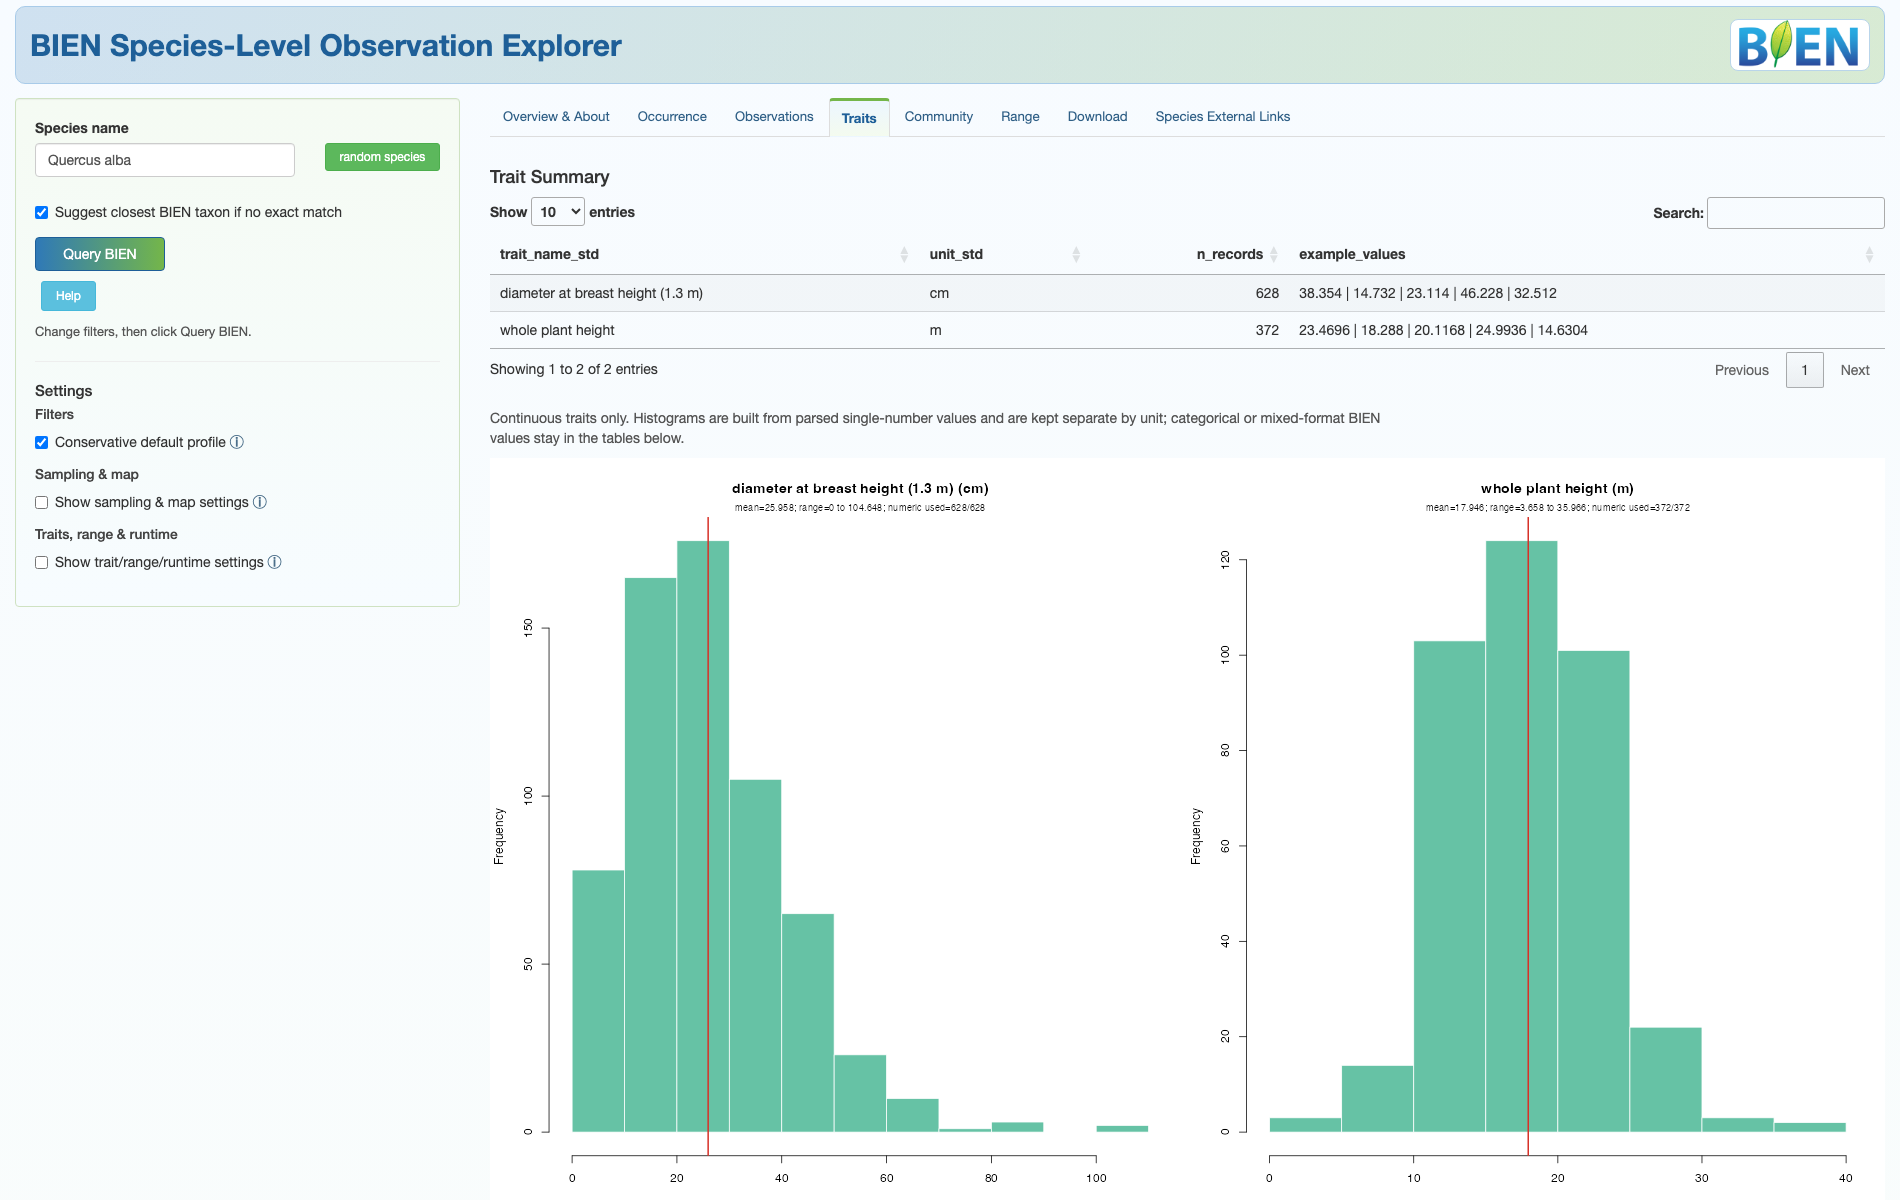
\includegraphics[width=\textwidth,height=0.78\textheight,keepaspectratio]{figures/fig_trait_data.png}
\caption{Traits view of the BIEN Species Shiny App for \textit{Pinus ponderosa} (locked screenshot species). The figure shows populated trait records in the data table, allowing direct inspection of trait names, values, and units for downstream analysis decisions.}
\label{fig:trait_data}
\end{figure}

\begin{figure}[htbp]
\centering
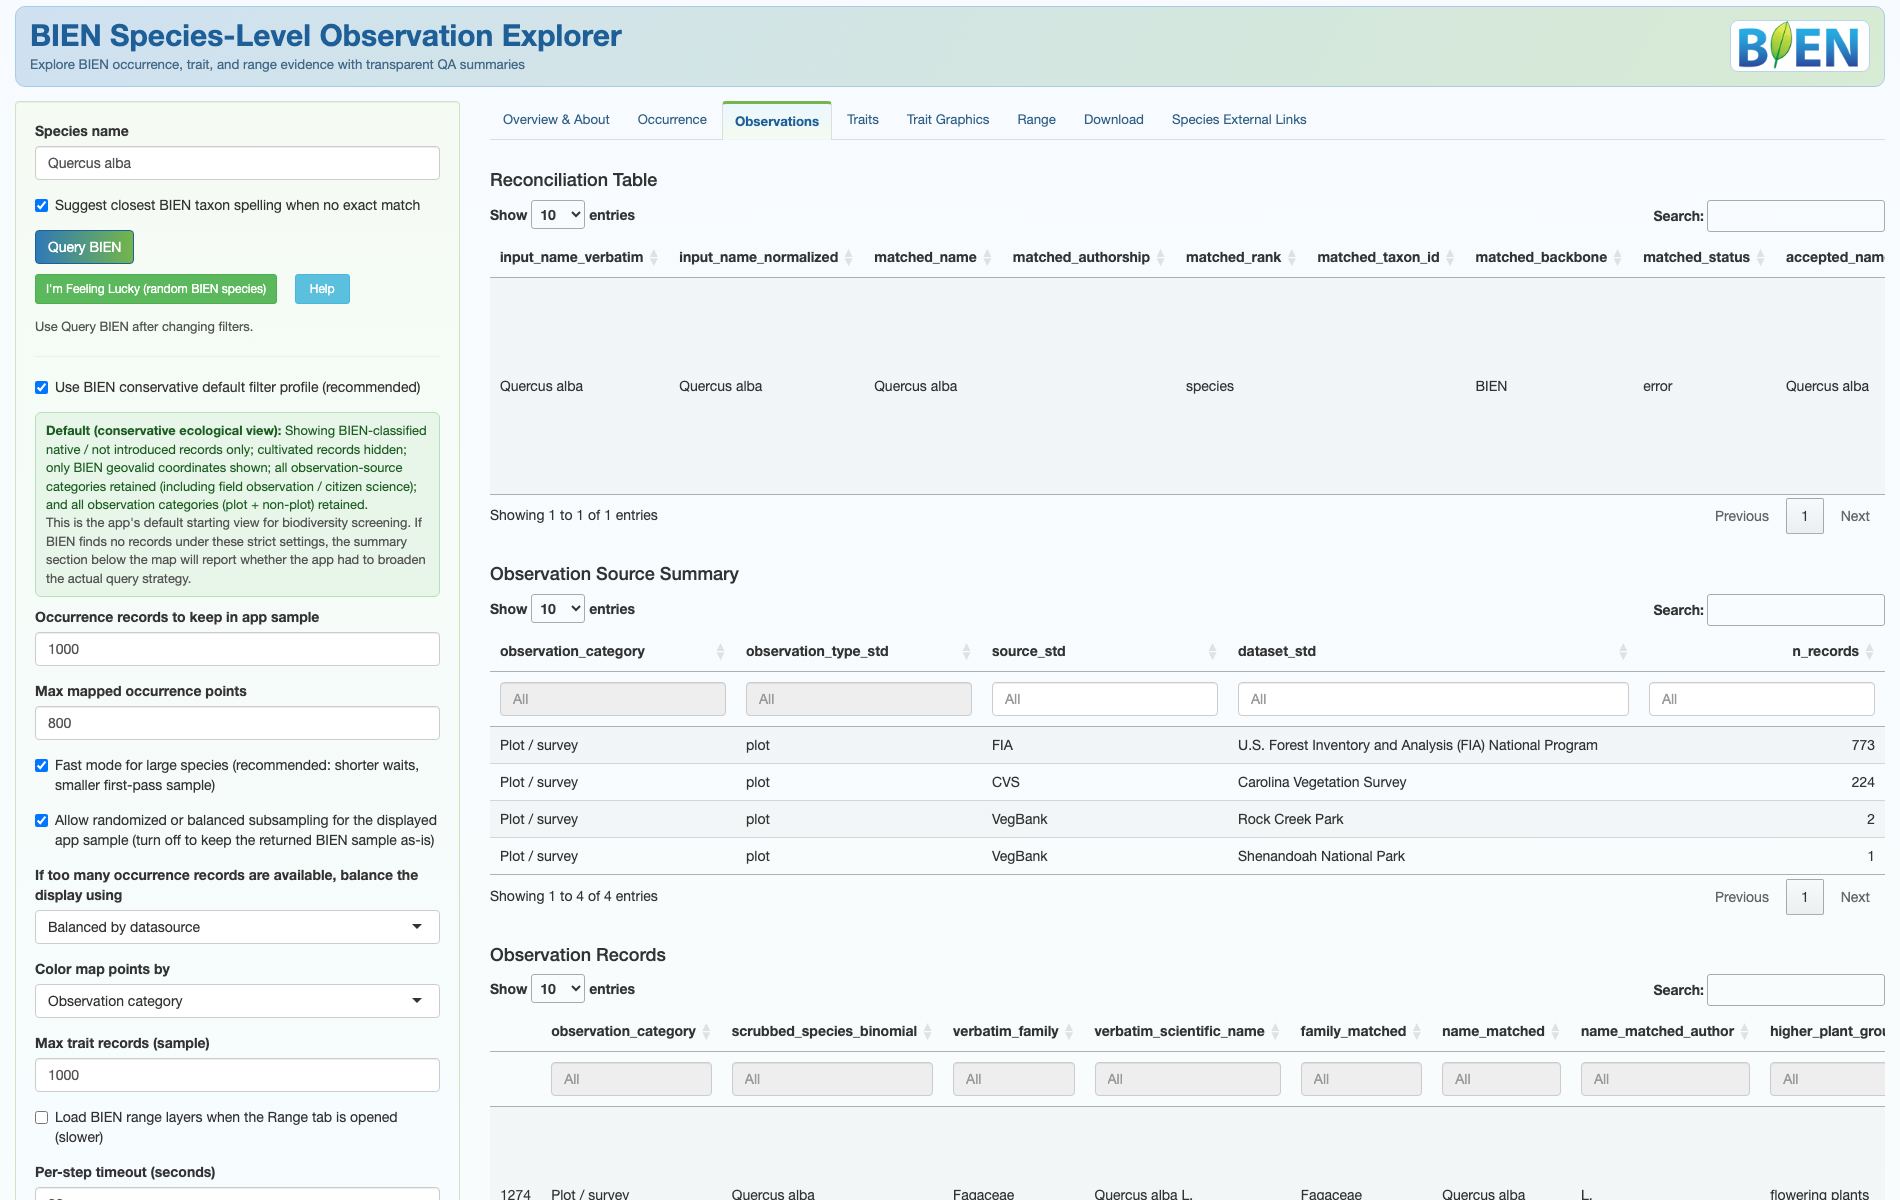
\includegraphics[width=\textwidth,height=0.72\textheight,keepaspectratio]{figures/fig_summary_stats.png}
\caption{Summary Statistics section (bottom of the Observations tab) for \textit{Pinus ponderosa}. This panel reports BIEN total counts, source-fraction context, active filters, query strategy, and mapped-point QA diagnostics for interpretation and reproducibility.}
\label{fig:summary_stats}
\end{figure}

\section*{How to use the app in practice}
The workflow is most effective when users follow the same sequence each time:
\begin{enumerate}
\item Define the ecological question before querying (for example: native-range screening, trait availability check, or broad occurrence reconnaissance).
\item Run a baseline query with the conservative default filters and inspect the Occurrence tab first (map plus overview diagnostics).
\item Check source composition and row-level provenance in the Observations tab, then review the Summary Statistics section at the bottom of that tab for BIEN totals, source fractions, and QA context.
\item Open the Community tab to inspect plot/survey-only mapped records and summary statistics when community-context evidence is important for the question.
\item Review the Traits tab (summary table plus raw records) and Trait Graphics tab to evaluate sample size, value format, and unit consistency for focal traits.
\item Inspect Range only as supporting context, not as a direct replacement for point-based occurrence evidence.
\item Use the Download tab to export occurrence, plot/community, and trait datasets plus reproducible BIEN query code, then archive active filters and query strategy in methods notes or supplementary files.
\end{enumerate}

In practice, this six-step flow helps prevent two common analysis errors. The first is overconfidence from large raw totals: a species can have many returned rows but still have limited high-quality, georeferenced, biologically relevant evidence after filtering. The second is silent scope drift: users may change filters while exploring and then forget which settings produced the final evidence pool. The app reduces both problems by keeping filters visible and by explicitly reporting fallback behavior when strict settings fail.

For team projects, it is useful to run the sequence twice for each focal species: once under conservative ecological filters and once under a broader evidence profile. Comparing these two passes reveals how sensitive conclusions are to introduced/cultivated handling, coordinate filtering, and source composition. If inferred distribution patterns, trait summaries, or record-source dominance change strongly between passes, that sensitivity should be reported and incorporated into downstream model interpretation. This comparison is fast to run but often highly informative for transparent study design.

\section*{Methodological value for ecology workflows}
\subsection*{Upstream quality screening before modeling}
A key contribution of the app is process, not a new model. It standardizes early checks that are often skipped in methods reporting: source composition, coordinate quality, filter rationale, and trait-format issues. This supports a cleaner handoff to formal analyses such as SDMs, where model results are sensitive to data cleaning choices and background assumptions \citep{Merow2013MaxEntGuide, Merow2014Maxlike}.

\subsection*{Interpretation-aware handling of heterogeneity}
By exposing filter toggles and category summaries directly in the interface, the tool encourages explicit choices rather than hidden defaults. Native/introduced and cultivated/wild distinctions are not universally required, but when they are relevant they materially alter inference targets. Making those controls visible helps align data retrieval with ecological question framing.

\subsection*{Communication and team science benefits}
The app is especially useful in collaborative settings where field ecologists, modelers, data stewards, and trainees need a shared diagnostic view before coding-heavy analysis begins. A common visual and tabular dashboard reduces ambiguity in project kickoff discussions and can improve consistency in documented inclusion criteria.

\section*{Reproducibility and transparency considerations}
The BIEN Species Shiny App improves transparency by making query behavior inspectable, but reproducibility still depends on upstream service state and package versions. BIEN-backed results can change as source datasets and taxonomic treatments evolve \citep{Enquist2026BIEN, Maitner2025BIEN}. Therefore, users should archive query dates, package versions, filter settings, and reconciliation outputs.

The app also includes performance-oriented choices (timeouts, sample caps, optional deferred loading for slower summaries/range queries). These features keep interactive use responsive, but users should distinguish between displayed samples and full matching pools. Optional count-only summary retrieval helps by providing denominator context for mapped fractions.

\section*{Limitations and guardrails}
First, the app is an exploratory screen, not a substitute for study-specific data cleaning and validation. Users should still run dedicated QA/QC steps before publication-level analyses.

Second, source categories are practical shortcuts and can misclassify records when metadata are sparse or inconsistent. They are designed to speed inspection, not to serve as final data standards.

Third, trait harmonization in the interface is intentionally light. The app highlights values, units, and distributions but does not perform full cross-source unit reconciliation. Those tasks remain part of downstream analysis.

Fourth, range layers are useful context but should not be treated as definitive occupancy boundaries without added evidence.

Finally, because the app emphasizes transparent defaults and fallback behavior, users should report actual query strategies used for each species rather than only nominal settings. This is crucial when strict filters yield no records and relaxed fallbacks are invoked.

\section*{Positioning within current methods development}
Ecology methods increasingly emphasize reproducible, data-aware workflows that begin with explicit inspection of evidence structure rather than immediate model execution. In this context, the BIEN Species Shiny App can be viewed as a boundary tool: it connects broad biodiversity cyberinfrastructure with practical, question-driven exploratory analysis. It offers a consistent entry point that is understandable to coders and non-coders alike, while preserving enough audit information for rigorous reporting.

This positioning is also compatible with contemporary work on model transferability and data integration. Methods guidance for SDMs repeatedly shows that model quality is constrained by input data assumptions and bias structure \citep{Merow2013MaxEntGuide, Merow2016ExpertMaps}. A lightweight pre-model inspection layer can therefore improve downstream methodological choices even when it introduces no new inferential algorithm itself.

\section*{Reproducible dataset code export}
Rather than relying on narrative reporting rules, the app now provides direct code export to reproduce the exact datasets shown in the app tables. In the \textit{Download} tab, users can download linked outputs for occurrence, plot/community, and trait retrievals: CSV exports of the current tables plus R scripts that reproduce those same pulls from BIEN using the same strategy and filters used in the app run.

The exported script includes a plain-language summary at the top that states the species queried, the BIEN strategy used (including fallback behavior if it occurred), the effective BIEN query flags, and app-side post-query filters. It then runs the same filtering and sampling logic used to build the displayed/downloaded table. This makes reproducibility practical because collaborators can regenerate the table from code, inspect each transformation step, and verify that a manuscript dataset matches app behavior.

This code-first export also helps review and handoff across teams. Instead of reconstructing settings from memory, users can archive the CSV and script pair as supplementary materials and rerun the script in a clean session. The result is a more direct and auditable bridge from interactive exploration to documented analysis \citep{Enquist2026BIEN, Maitner2025BIEN}.

\section*{Conclusions}
The BIEN Species Shiny App provides a practical, transparent framework for species-level evidence triage across occurrence, trait, and range dimensions. Its strength lies in explicit interpretation support: users can see what evidence exists, what filters shape that evidence, and where uncertainty or heterogeneity may affect analysis design. For projects using BIEN as a central data source, the app offers a reproducible front-end step that can improve communication, reduce hidden assumptions, and inform better downstream modeling decisions.

In short, this tool operationalizes a simple but consequential methods principle: inspect data-generating context before inference. As biodiversity workflows continue to scale, interfaces that make provenance and filter logic visible will remain essential for robust ecological science.

\bibliographystyle{apalike}
\bibliography{references}

\section*{Word count}
Main text word count (texcount, excluding references): 1897 words.

\end{document}
